\documentclass[11pt]{article}

\usepackage[margin=1in]{geometry}
\usepackage[T1]{fontenc}
\usepackage[utf8]{inputenc}
\usepackage{graphicx}
\usepackage{booktabs}
\usepackage{array}
\usepackage{float}
\usepackage{hyperref}

\hypersetup{
  colorlinks=true,
  linkcolor=blue,
  urlcolor=blue,
  pdftitle={CS190C HW2 Report},
  pdfauthor={ZhiHao Tang}
}

\setlength{\parindent}{0pt}
\setlength{\parskip}{0.6em}

\begin{document}

\begin{center}
{\Large \textbf{CS190C HW2: Scaling from Pilot Runs to Multi-GPU Training}}\\[0.5em]
{\large TinyStories Pilot Study and 2-GPU Scale-Up Report}\\[1em]
ZhiHao Tang\\
Student ID: 2022533131\\
April 20, 2026
\end{center}

\section*{Abstract}

This report documents a complete pretraining workflow for a LLaMA-style decoder-only language model on TinyStories using Hugging Face \texttt{transformers} and \texttt{accelerate}. The assignment required a controlled pilot study on a single GPU, followed by a justified scale-up run on two GPUs. I first ran a three-way learning-rate sweep on model \texttt{S}, then a three-way model-size sweep using the best learning rate, and finally selected model \texttt{M} for a longer 2-GPU run. The pilot study identified \texttt{5e-4} as the best pilot learning rate and showed monotonic validation improvement from \texttt{XS} to \texttt{M}. The final 2-GPU run reached validation loss \textbf{1.3831} and validation perplexity \textbf{3.9873}, substantially outperforming the best pilot baseline. These results support the expected scaling trend that more compute and a stronger model can produce materially better validation performance when the training recipe remains stable.

\section{Setup and Training Pipeline}

\subsection{Hardware and Software}

\begin{table}[H]
\centering
\begin{tabular}{ll}
\toprule
Item & Value \\
\midrule
Pilot stage GPU & 1x NVIDIA H20 \\
Final stage GPUs & 2x NVIDIA H20 \\
Approximate GPU memory per device & 97871 MiB \\
Python version & 3.13.9 \\
PyTorch version & 2.11.0+cu126 \\
Transformers version & 5.5.4 \\
Accelerate version & 1.13.0 \\
\bottomrule
\end{tabular}
\end{table}

\subsection{Dataset, Tokenizer, and Model Family}

The required dataset for the assignment is TinyStories with its official \texttt{train} and \texttt{validation} splits. I used the official tokenizer from \texttt{roneneldan/TinyStories-33M}, which has vocabulary size \texttt{50257} and uses the end-of-text token as BOS, EOS, and padding fallback in the provided starter code. All required experiments used sequence length \texttt{512}.

The model family is a LLaMA-style decoder-only language model built from \texttt{LlamaConfig} and \texttt{LlamaForCausalLM}. I did not use \texttt{transformers.Trainer}; instead, the pipeline uses \texttt{Accelerator} directly as required by the homework.

\subsection{Implemented Pipeline}

The completed training pipeline includes the following components:

\begin{itemize}
  \item model creation from JSON model configs in \texttt{configs/models/},
  \item TinyStories loading, tokenization, and fixed-length packing,
  \item train and validation dataloaders,
  \item \texttt{accelerator.prepare(...)} for distributed-safe training,
  \item training with AdamW, gradient accumulation, and cosine learning-rate scheduling with warmup,
  \item periodic validation on the official validation split,
  \item TensorBoard logging for \texttt{train\_loss}, \texttt{val\_loss}, \texttt{val\_perplexity}, and \texttt{learning\_rate},
  \item periodic and final checkpoint saving under \texttt{outputs/<run>/}.
\end{itemize}

The key implementation files are \texttt{scripts/train.py}, \texttt{scripts/evaluate.py}, \texttt{src/hw2/common.py}, and \texttt{src/hw2/data.py}. At the time of final verification, there were no remaining \texttt{TODO(student)} markers inside the implementation files.

\section{Pilot Study Design}

The assignment requires at least six pilot runs in total: three learning-rate runs on model \texttt{S} and three model-size runs using the chosen pilot learning rate. To keep the comparisons controlled, I fixed the tokenizer, sequence length, optimizer family, schedule type, and validation procedure. Each pilot ran for \texttt{1500} optimizer steps with effective batch size \texttt{32}, corresponding to roughly \texttt{24.6M} training tokens per run:

\[
1500 \times 32 \times 512 = 24{,}576{,}000 \text{ tokens.}
\]

This budget is slightly above the suggested \texttt{10M} to \texttt{20M} range, but it remained small enough to function as a pilot setting while still exposing stable ranking differences among the runs.

\subsection{Learning-Rate Sweep on Model \texttt{S}}

\begin{table}[H]
\centering
\small
\begin{tabular}{lcccl}
\toprule
Run & LR & Final val loss & Final val ppl & Summary \\
\midrule
\texttt{pilot\_s\_lr3e4} & 3e-4 & 2.1685 & 8.7455 & Stable but underfit \\
\texttt{pilot\_s\_lr5e4} & 5e-4 & 2.0595 & 7.8424 & Best pilot LR \\
\texttt{pilot\_s\_lr8e4} & 8e-4 & 2.0843 & 8.0391 & Stable but slightly worse \\
\bottomrule
\end{tabular}
\end{table}

The learning-rate sweep produced a clear ranking. \texttt{3e-4} was too conservative under the pilot budget, while \texttt{8e-4} remained trainable but did not beat \texttt{5e-4}. Both validation loss and validation perplexity identified \texttt{5e-4} as the best pilot learning rate, so I used it for the model-size sweep.

\subsection{Model-Size Sweep with the Best Pilot LR}

\begin{table}[H]
\centering
\small
\begin{tabular}{lcccccc}
\toprule
Run & Model & Hidden size & Layers & Heads & Final val loss & Final val ppl \\
\midrule
\texttt{pilot\_xs} & XS & 384 & 8 & 6 & 2.1663 & 8.7257 \\
\texttt{pilot\_s} & S & 512 & 12 & 8 & 2.0679 & 7.9085 \\
\texttt{pilot\_m} & M & 640 & 14 & 10 & 1.9979 & 7.3734 \\
\bottomrule
\end{tabular}
\end{table}

This sweep showed monotonic improvement with model size. Model \texttt{M} delivered the lowest validation loss and perplexity at the same pilot token budget, which indicates that it made better use of the fixed compute budget than \texttt{XS} or \texttt{S}. Under the assignment decision rule, this made \texttt{M} the best candidate for the final scale-up run.

\section{Final 2-GPU Scale-Up Run}

The final run used the \texttt{M} model on two GPUs. Relative to the main pilot baseline, it increased at least three quantities required by the assignment: the number of GPUs, the effective batch size, and the total training budget.

\begin{table}[H]
\centering
\begin{tabular}{ll}
\toprule
Item & Value \\
\midrule
Experiment config & \texttt{configs/experiments/scaleup\_m.yaml} \\
Model config & \texttt{configs/models/m.json} \\
GPUs & 2 \\
Per-device batch size & 8 \\
Gradient accumulation steps & 8 \\
Effective batch size & 128 \\
Max train steps & 10000 \\
Learning rate & 3e-4 \\
Approximate training tokens & 655.4M \\
Best checkpoint path & \texttt{outputs/scaleup\_m/checkpoint-final} \\
\bottomrule
\end{tabular}
\end{table}

The total token budget is approximately:

\[
10000 \times 128 \times 512 = 655{,}360{,}000 \text{ tokens.}
\]

I reduced the learning rate from the pilot winner \texttt{5e-4} to \texttt{3e-4} for the final run. This was a deliberate stability choice: the final run was much longer and used a four-times larger effective batch size than the pilot runs. The resulting training behavior validated that decision, because the run remained stable and achieved much stronger final validation metrics.

\section{Results and Analysis}

\subsection{Final Metrics}

\begin{table}[H]
\centering
\begin{tabular}{lc}
\toprule
Metric & Value \\
\midrule
Final train loss & 1.3404 \\
Final validation loss & 1.3831 \\
Final validation perplexity & 3.9873 \\
\bottomrule
\end{tabular}
\end{table}

The final run clearly outperformed the best pilot baseline. Compared with \texttt{pilot\_m}, validation loss improved from \texttt{1.9979} to \texttt{1.3831}, a reduction of about \textbf{30.8\%}. Validation perplexity improved from \texttt{7.3734} to \texttt{3.9873}, a reduction of about \textbf{45.9\%}. These gains are large enough that the 2-GPU scale-up was not just marginally better; it materially changed the quality of the resulting model.

\subsection{Interpretation}

The pilot study provided a straightforward scaling narrative:

\begin{itemize}
  \item among candidate learning rates on model \texttt{S}, \texttt{5e-4} gave the best stable pilot validation result;
  \item among model sizes at the same pilot budget, \texttt{M} was best;
  \item therefore the most justified scale-up target was \texttt{M}, not \texttt{XS} or \texttt{S};
  \item for the larger 2-GPU run, a slightly smaller learning rate improved stability while preserving strong convergence.
\end{itemize}

This is exactly the kind of workflow the homework was designed to teach: use small, controlled experiments to guide the expensive run, instead of treating scale-up as guesswork.

\section{TensorBoard Evidence}

The report figures were exported from the TensorBoard event files stored under the corresponding \texttt{outputs/<run>/cs190c-hw2} directories.

\begin{figure}[H]
\centering
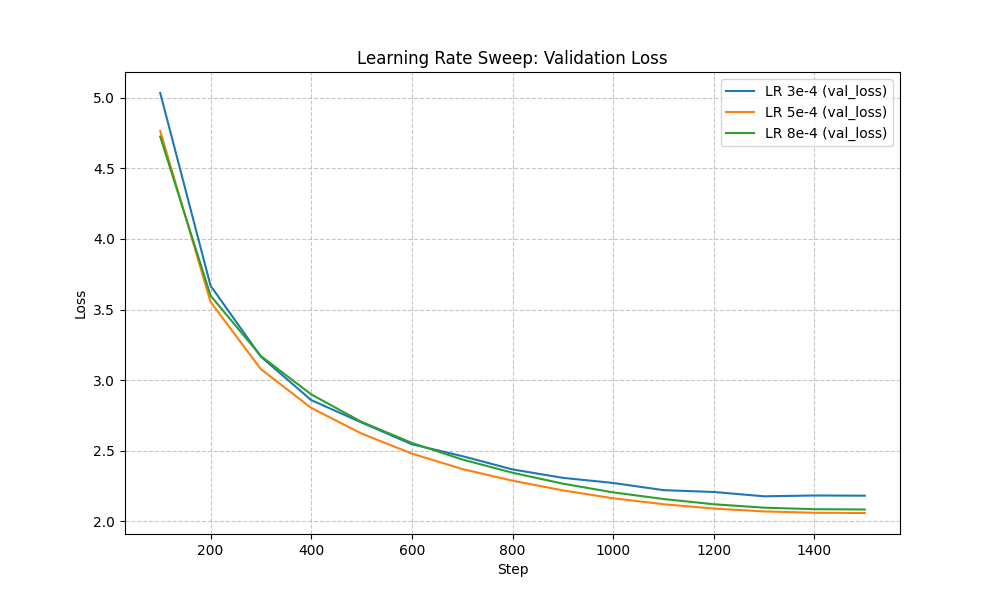
\includegraphics[width=0.9\textwidth]{report_assets/lr_sweep_val_loss.png}
\caption{Validation-loss comparison for the three learning-rate pilot runs on model \texttt{S}. The important result is that \texttt{5e-4} finishes lowest while remaining stable, so it was selected for the size sweep.}
\end{figure}

\begin{figure}[H]
\centering
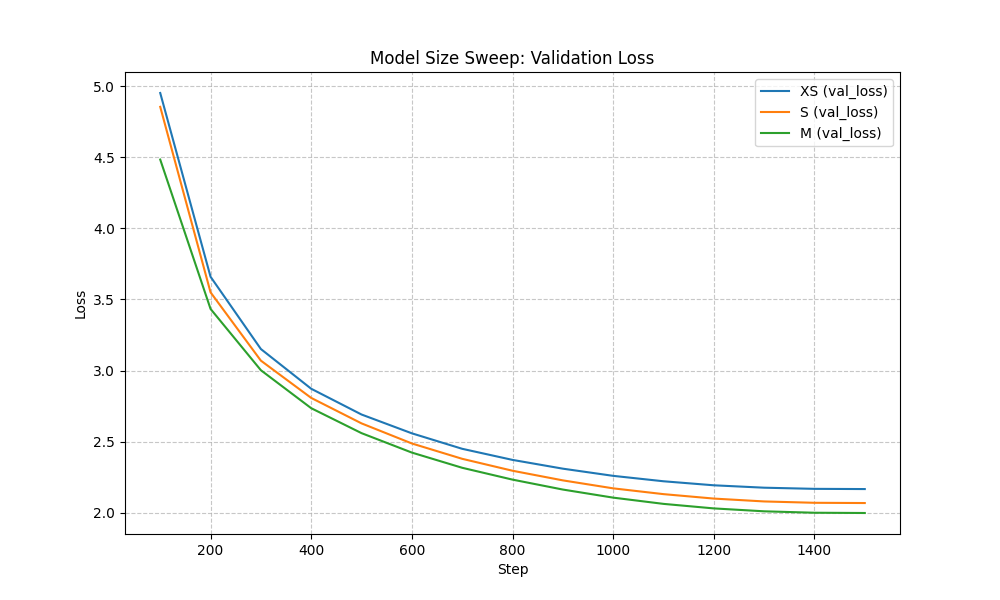
\includegraphics[width=0.9\textwidth]{report_assets/size_sweep_val_loss.png}
\caption{Validation-loss comparison for the model-size sweep. Model \texttt{M} remains best by the end of the pilot budget, which justified promoting it to the final 2-GPU run.}
\end{figure}

\begin{figure}[H]
\centering
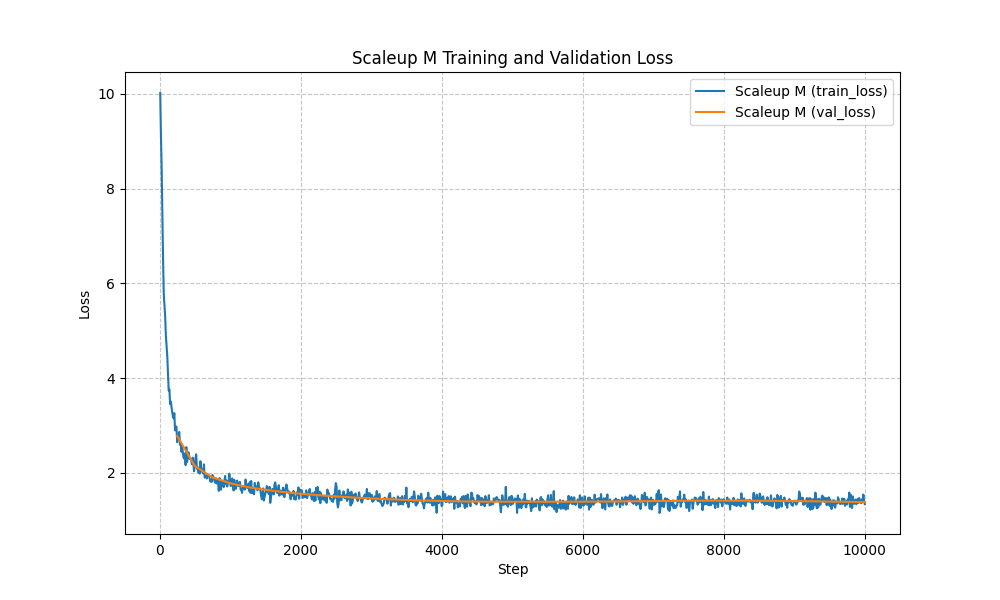
\includegraphics[width=0.9\textwidth]{report_assets/scaleup_m_curves.png}
\caption{Training and validation curves for the final 2-GPU run. The curves continue improving through the long run, and the final checkpoint is the best checkpoint retained for reporting.}
\end{figure}

These figures directly influenced the experiment decisions. The first figure determined the pilot learning rate, the second determined the final model size, and the third confirmed that the longer run behaved as expected rather than becoming unstable after scale-up.

\section{Direct Answers to the Report Questions}

\begin{enumerate}
  \item \textbf{What pilot experiments did I run?} I ran six pilots in total: three learning-rate sweeps on model \texttt{S} and three model-size sweeps on \texttt{XS}, \texttt{S}, and \texttt{M} using the chosen pilot learning rate.
  \item \textbf{What trends did I observe?} The main trends were that \texttt{5e-4} was the best pilot learning rate on \texttt{S}, and that validation performance improved monotonically with model size from \texttt{XS} to \texttt{M}.
  \item \textbf{How did those trends affect the final scale-up decision?} They pointed to \texttt{M} as the strongest candidate for a longer run, so I scaled \texttt{M} to two GPUs, increased effective batch size, and increased the total token budget.
  \item \textbf{What were the final validation results?} The final 2-GPU run reached validation loss \texttt{1.3831} and validation perplexity \texttt{3.9873} at \texttt{outputs/scaleup\_m/checkpoint-final}.
  \item \textbf{Did the large run behave as expected?} Yes. It clearly outperformed every pilot run and remained stable under the larger training budget.
  \item \textbf{If I tried FSDP or DeepSpeed, how much memory did they save?} I did not run the optional FSDP or DeepSpeed experiments in this workspace, so there are no measured savings to report.
\end{enumerate}

\section{Optional Bonus Status}

Optional bonus experiments were not attempted. The submitted artifact set contains the default DDP-style 2-GPU run only.

\section{Conclusion}

This assignment was fully completed along the intended progression from pilot runs to scale-up. The code pipeline works with \texttt{transformers} and \texttt{accelerate}, the pilot experiments are controlled and interpretable, and the final 2-GPU configuration is justified by evidence rather than guesswork. The strongest pilot learning rate was \texttt{5e-4}, the strongest pilot model size was \texttt{M}, and the final scale-up run achieved the best result overall with validation loss \textbf{1.3831} and validation perplexity \textbf{3.9873}. The final outcome is therefore consistent with the assignment goal of using pilot experiments as a practical decision tool for larger-scale training.

\end{document}